%% ===================================================================
\section{Multivariate Regression}
\label{sec:regression}
Multivariate regressors are capable of accurately modeling a complex
dependence of a response (in $Y$) on multiple variables (represented
as a points in $\mathbb{R}^{d}$). The approximations to some (unknown)
underlying function $f: \mathbb{R}^d \rightarrow Y$ are chosen to
minimize some error measure related to data samples
$f\bigl(x^{(i)}\bigr)$. For example, least squares regression uses the
sum of squared differences between modeled function values and true
function values as an error measure. In this section and the next,
some techniques are limited to approximating real valued functions ($Y
\subset \mathbb{R}$). These techniques can be extended to real
vector-valued ranges by repeating the construction for each component
of the vector output. Throughout the following, $x$ denotes a
$d$-tuple, $x_i$ the $i$th component of $x$, and $x^{(i)}$ the $i$th
$d$-tuple data point. Different symbols are used to represent the
approximation function $\hat f$.

\subsection{Multivariate Adaptive Regression Splines}
\label{sec:mars}
This approximation was introduced in \cite{friedman1991multivariate}
and subsequently improved to its current version in
\cite{stanford1993fast}, called fast multivariate adaptive regression
splines (Fast MARS). In Fast MARS, a least squares fit model is
iteratively built by beginning with a single constant valued function
and adding two new basis functions at each iteration of the form
\begin{align*}
  B_{2j-1}(x) &= B_l(x) \bigl(x_i-x^{(p)}_i\bigr)_+, \\
  B_{2j}(x) &= B_k(x) \bigl(x_i-x^{(p)}_i\bigr)_- ,
\end{align*}
where $j \leq m$ is the iteration number, $m$ is the maximum
  number of underlying basis functions, $1 \le p \le n$, and
$B_l(x)$, $B_k(x)$ are basis functions from the previous iteration,
 $$w_+ = \begin{cases} w, & w \geq 0 \\ 0, & w < 0 \end{cases},$$ and
$w_- = (-w)_+$. After iteratively constructing a model, MARS then
iteratively removes basis functions that do not contribute to goodness
of fit. In effect, MARS creates a locally component-wise tensor
product approximation of the data. The overall computational
complexity of Fast MARS is $\mathcal{O}(n d m^3)$. This work
uses an implementation of Fast MARS \cite{rudy2017pyearth} with $m =
200$ throughout all experiments.

\subsection{Support Vector Regressor}
\label{sec:svr}
Support vector machines are a common method used in machine learning
classification tasks that can be adapted for the purpose of regression
\cite{basak2007support}. How to build a support vector regressor (SVR)
is beyond the scope of this summary, but the resulting functional fit
$p : \mathbb{R}^d \rightarrow \mathbb{R}$ has the form
 $$ p(x)  = \sum_{i=1}^{n}a_i K\bigl(x,x^{(i)}\bigr) + b ,$$
where $K$ is the selected kernel function, $a_i \in \mathbb{R}^n$, 
$b \in \mathbb{R}$ are coefficients to be solved for simultaneously.
The computational complexity of the SVR is $\mathcal{O}(n^2dm)$, with
$m$ being determined by the minimization convergence criterion. This
work uses the scikit-learn SVR \cite{scikit-learn} with a radial
basis function kernel.

\subsection{Multilayer Perceptron Regressor}
\label{sec:mlp}
The neural network is a well studied and widely used method for both
regression and classification tasks
\cite{hornik1989multilayer,rumelhart1988learning}. When using the
rectified linear unit (ReLU) activation function
\cite{dahl2013improving} and fitting the model with stochastic
gradient descent (SGD) or BFGS minimization techniques
\cite{goh2017why,moller1993scaled,robbins1951stochastic}, the model
built by a multilayer perceptron uses layers $l : \mathbb{R}^{i}
\rightarrow \mathbb{R}^{j}$ defined by
 $$ l(u) = \bigl( u^t W_l + c_l \bigr)_+ ,$$
where $c_l \in \mathbb{R}^j$ and $W_l$ is the $i \times j$ weight
matrix for layer $l$. In this form, the multilayer perceptron (MLP)
produces a piecewise linear model of the input data. The computational
complexity of training a multilayer perceptron is $\mathcal{O}(n d
m)$, where $m$ is determined by the sizes of the layers of the network
and the stopping criterion of the minimization used for finding
weights. This work uses an MLP built from Keras and Tensorflow to
perform regression \cite{tensorflow2015-whitepaper,chollet2015keras}
with ten hidden layers each having thirty two nodes (a total of
approximately ten thousand parameters), ReLU activation, and
one hundred thousand steps of SGD
for training. It should be noted that the choice of neural
  network architecture affects approximation performance, but no
  architecture tuning is performed here.

%% ===================================================================
\section{Multivariate Interpolation}
\label{sec:interpolation}
The following interpolation techniques demonstrate a reasonable
variety of approaches to interpolation. All of the presented
interpolants produce approximations that are continuous in value,
which is often a desirable property in applied approximation problems.

\subsection{Delaunay}
\label{sec:delaunay}

The Delaunay triangulation is a well-studied geometric technique for
producing an interpolant \cite{lee1980two}. The Delaunay triangulation
of a set of points into simplices is such that there
are no points inside the sphere defined by the
vertices of each simplex. For a $d$-simplex S with vertices $x^{(0)}$,
$x^{(1)}$, $\ldots$, $x^{(d)}$, and function values
$f\bigl(x^{(i)}\bigr)$, $i=0$, $\ldots$, $d$, $y \in S$ is a unique
convex combination of the vertices,
 $$ y = \sum_{i=0}^{d} w_i x^{(i)}, \quad \sum_{i=0}^{d} w_i = 1, \quad w_i \geq 0, \quad i=0,\ldots,d, $$
and the Delaunay interpolant $\hat f(y)$ at $y$ is given by
 $$ \hat f(y) = \sum_{i=0}^{d} w_i f\bigl(x^{(i)}\bigr). $$ The
computational complexity of Delaunay interpolation (for the
implementation used \cite{chang2018polynomial}) is $\mathcal{O}(k n
d^3)$. Given pathological data the entire triangulation could be
computed with $k = n^{\lceil d / 2 \rceil}$, but the average case yields
$k = d \log d$ and is capable of scaling reasonably to $d \leq 50$. In
the present application, a Delaunay simplex $S$ containing $y$ is
found, then the $d+1$ vertices (points in $X$) of $S$ are used to
assign weights to each vertex and produce the predicted function value
for point $y$.

\begin{figure}
  \centering
  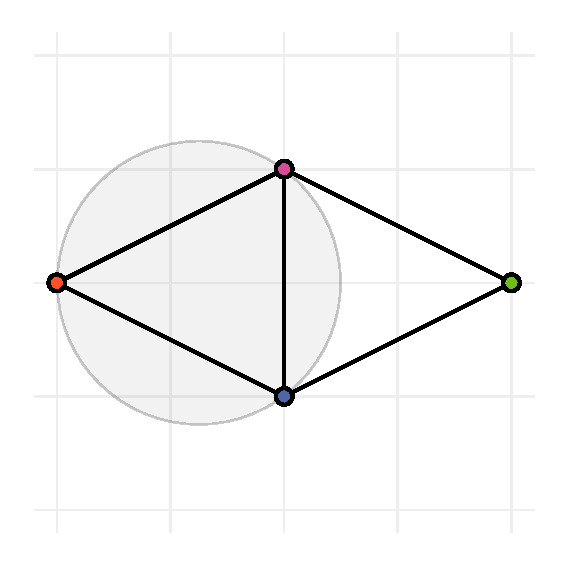
\includegraphics[width=0.4\textwidth,]{Figures/NA/example_delaunay.pdf}
  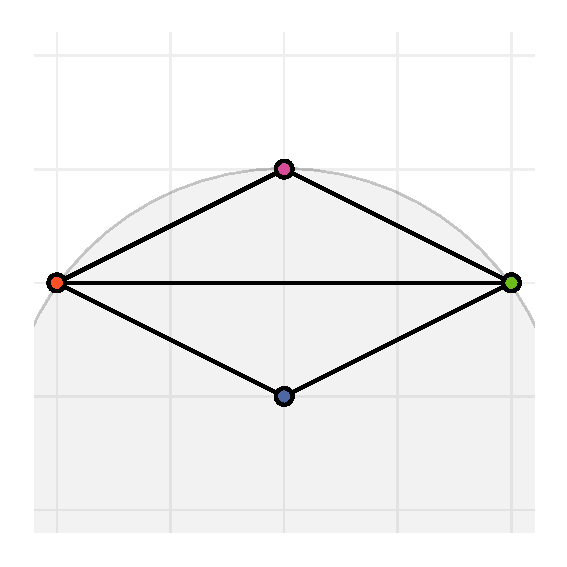
\includegraphics[width=0.4\textwidth,]{Figures/NA/example_not_delaunay.pdf}
  \caption{On the left above is a depiction of a Delaunay
    triangulation over four points, notice that the circumball (shaded
    circle) for the left simplex does not contain the fourth point.
    On the right above, a non-Delaunay mesh is depicted. Notice that
    the circumball for the top simplex (shaded circle, clipped at
    bottom edge of the visual) contains the fourth point which
    violates the Delaunay condition for a simplex.
  \vspace{-.1cm}}
  \label{fig:delaunay}
\end{figure}


\subsection{Modified Shepard}
\label{sec:modified-shepard}

The modified Shepard method used here (ShepMod) generates a continuous
approximation based on Euclidean distance and resembles a nearest
neighbor interpolant \cite{cover1967nearest}. This model is a type of
\textit{metric interpolation}, also called a Shepard method
\cite{gordon1978shepard,shepard1968two}. The interpolant has the form
 $$ p(x) = \frac{\sum\limits_{k=1}^{n}W_k(x)f\bigl(x^{(k)}\bigr)}
     {\sum\limits_{k=1}^{n}W_k(x)} ,$$ where
     $p\bigl(x^{(k)}\bigr) = f\bigl(x^{(k)}\bigr)$, $W_k(x) =
       \bigl(\bigl(r_k - \bigl\|x - x^{(k)}\bigr\|_2\bigr)_+ \big/
       \bigl( r_k \bigl\|x - x^{(k)}\bigr\|_2 \bigr)\bigr)^2$ for $x
       \neq x^{(k)}$, and $r_k \in \mathbb{R}$ is the smallest
     radius such that at least $d+1$ other points $x^{(j)}$, $j \not =
     k$, are inside the closed Euclidean ball of radius $r_k$ about
     $x^{(k)}$. The interpolant $p(x)$ is continuous because
       the singularities at the $x^{(k)}$ are removable. The
     computational complexity of ShepMod is $\mathcal{O}(n^2d)$. This
     work uses a Fortran 95 implementation of ShepMod derived from
     SHEPPACK \cite{thacker2010algorithm}.

\begin{figure}
  \centering
  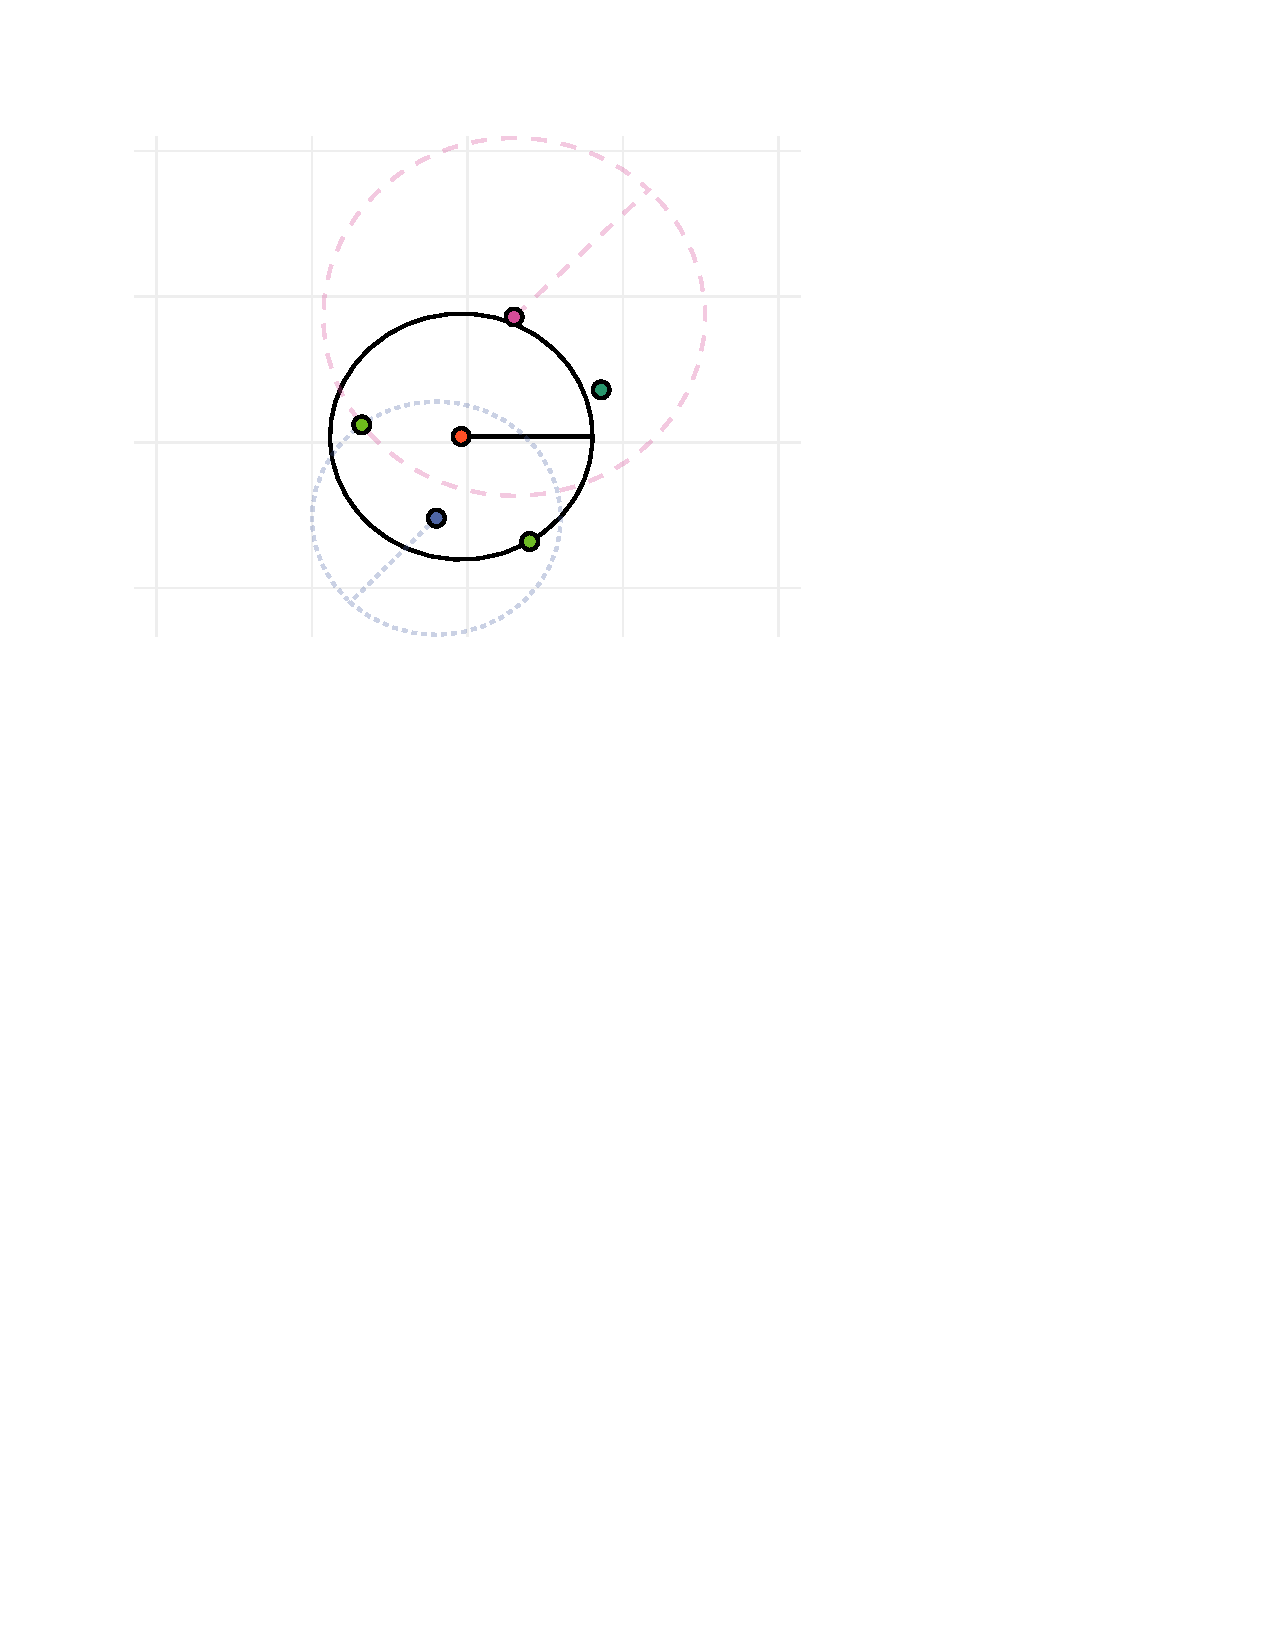
\includegraphics[width=0.4\textwidth,]{Figures/NA/example_shepard_radius.pdf}
  \hspace{.2cm}
  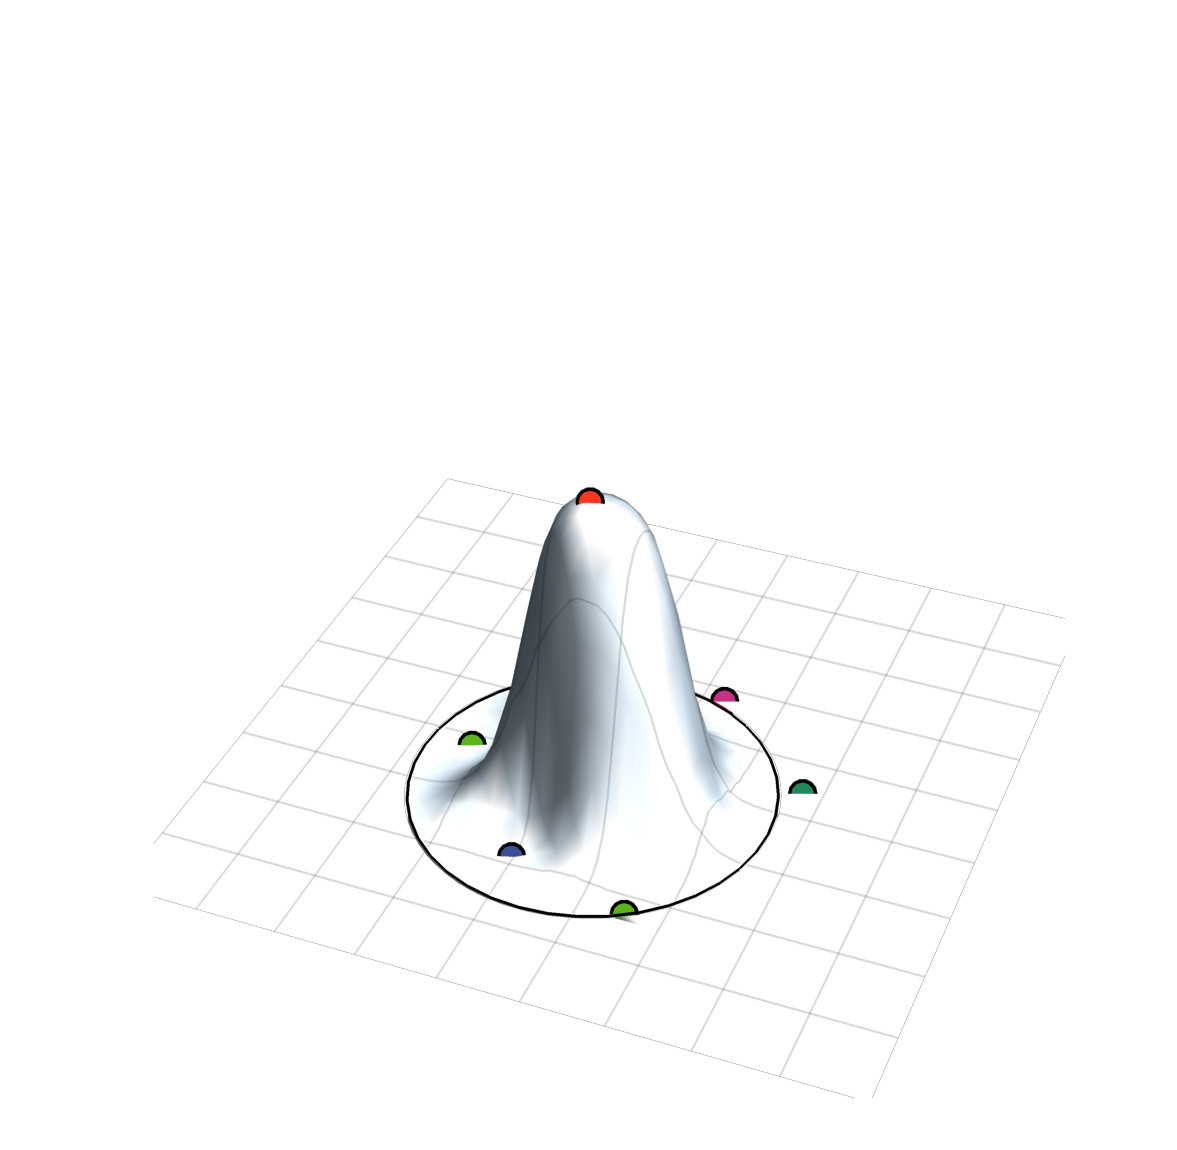
\includegraphics[width=0.4\textwidth,]{Figures/NA/example_shepard_weight.pdf}
  \caption{On the left above is a depiction of the radius
    of influence for three chosen points of a collection in two
    dimensions using the modified Shepard criteria. On the right a
    third axis shows the relative weight for the center most
    interpolation point $x^{(i)}$ with the solid line representing its
    radius of influence, where $W_i(x)$ is $0$ for $\|x-x^{(i)}\|_2
    \geq r_i$ and $W_i(x) / \sum_{k=1}^n W_k(x) \to 1$ as $x \to
    x^{(i)}$.
  \vspace{-.1cm}}
  \label{fig:shepard}
\end{figure}


\subsection{Linear Shepard}
The linear Shepard method (LSHEP) is a blending function using local
linear interpolants, a special case of the general Shepard algorithm
\cite{thacker2010algorithm}. The interpolant has the form
 $$ p(x) = \frac{\sum\limits_{k=1}^{n}W_k(x)P_k(x)}
 {\sum\limits_{k=1}^{n}W_k(x)} ,$$
where $W_k(x)$ is the same as for the modified Shepard method and
$P_k(x)$ is a local linear approximation to the data satisfying
$P_k\bigl(x^{(k)}\bigr) = f\bigl(x^{(x)}\bigr)$. The computational
complexity of LSHEP is $\mathcal{O}(n^2d^3)$. This work uses the
Fortran 95 implementation of LSHEP in SHEPPACK
\cite{thacker2010algorithm}.
